	
\documentclass{llncs}

\usepackage{booktabs}            % formatting of tables (lines, spacing)
\usepackage{tabularx}            % extended tables.
\usepackage{fancyvrb}
\usepackage{graphicx}
\usepackage{varioref}
\usepackage{enumerate}
\usepackage{url}
\urlstyle{sf}

\DefineVerbatimEnvironment{codeblock}{Verbatim}%
    {frame=lines,numbers=none,numbersep=0pt,fontsize=\scriptsize}

\newcommand{\tabcaption}[1]{\multicolumn{1}{c}{#1}}
\newcommand{\todo}[1]{\marginpar{\tiny #1}}

\newcommand{\internalsection}[1]{\par\medskip\noindent-- \emph{#1}~}

\newcommand{\customtextsc}[1]{{\scriptsize \MakeUppercase{#1}}}
\newcommand{\acro}[1]{\customtextsc{#1}}   % generic acronym
\newcommand{\gui}{\acro{gui}}              % GUI (acronym)
\newcommand{\jme}{\acro{j2me}}             % J2ME acronym

\newcommand{\method}[1]{\texttt{#1}}       % method name
\newcommand{\class}[1]{\texttt{#1}}        % class name
\newcommand{\interface}[1]{\texttt{#1}}    % interface name

\newcommand{\pcite}[1]{[\ref{#1}]}         % product citation


\begin{document}

\mainmatter

\title{Automated Integration Tests for Mobile~Applications in Java~2~Micro~Edition}

% Authors alphabetically; otherwise people have weird assumptions...
\author{Dawid Weiss \and Marcin Zduniak
\institute{Poznan University of Technology, Piotrowo 2, 60-965 Pozna{\'n}, Poland
\email{dawid.weiss@cs.put.poznan.pl}, \email{mzduniak@j2me.pl}}}

\maketitle              % typeset the title of the contribution

\begin{abstract} 
Applications written for mobile devices have become more and more complex, adjusting to the
constantly improving computational power of hardware. With the growing application size comes the
need for automated testing frameworks, particularly frameworks for automated testing of user
interaction and graphical user interface. While such testing (also called
\emph{capture-replay}) has been thoroughly discussed in literature with respect to desktop
applications, mobile development limits the possibilities significantly. To our best knowledge only
a few solutions for creating automated tests of mobile applications exist and their functionality
is very limited in general or constrained to only proprietary devices. 
In this paper we demonstrate preliminary results of our attempt to design and implement a
framework for capturing and replaying user interaction in applications written for the Java 2 Micro
Edition environment. Our evaluation test bed is a complex commercial mobile navigation system
and the outcomes so far are very promising.

\medskip\noindent\textbf{Keywords:~}Software~Testing, Agile~Development, Quality~Assurance, Mobile~Development 
\end{abstract}


\section{Introduction} % {{{

Software testing is a process of verifying the quality of computer programs to make sure they are
doing what was expected in a consistent, error-free manner. But software testing in practice depends
on \emph{how} and \emph{when} it takes place in the development process. We can distinguish several
types of tests~\cite{tcs,softqualiteng}. \emph{Unit testing} concentrates on low-level pieces of
software, such as classes and methods. These tests are typically a responsibility of the programmer
transforming the design into implementation. \emph{Acceptance tests} occur at the end of the
development process -- when the software is confronted with its initial requirements specification
and expectations of target users. \emph{Integration tests} (also called \emph{regression tests}),
which we focus on in this paper, happen in between unit and acceptance tests and cover larger blocks
of the program, often the entire product. By running integration tests frequently, we ensure all the
modules work together as a whole and provide results consistent with previously released versions of
the software. Regression tests are thus a quality control aspect -- they allow early detection 
of the program's suspicious behavior caused by changes (refactorings or new features) introduced to 
the product. This kind of constant software testing in anticipation of potential errors is part of most modern 
software development methodologies and is called the \emph{continuous integration}~principle~\cite{fowler}.

While theoretically appealing, writing integration tests for applications with a rich graphical user
interface (\gui{}) presents a generally complex technical problem. Since the human-computer
interaction is quite unpredictable, \gui{} applications resist rigorous testing.
A common solution is to \emph{record} real scenarios of user interaction with the program (directly
off the application's screen) and then try to reproduce the same stimuli at the testing phase,
validating program's response accordingly. This kind of procedure is made possible with various
\gui{} automation tools and programming interfaces; programs for recording \gui{}
events are called \emph{robots} and the technique is dubbed \emph{capture-replay testing methodology}.

Java 2 Micro Edition environment (\jme{}) lacks most of the above facilities for implementing \gui{}
automation. All existing products (research or commercial) for testing mobile applications in \jme{}
are very simple and lack capture-replay testing support. This fact raises the following questions:
%
\begin{itemize}
    \item In spite of technical difficulties, is it possible to devise a cross-platform architecture 
	facilitating unit and integration testing of mobile applications? How much overhead (code, time) 
	is required for running such a solution?
    \item Is there an industry need for integration tests aimed for mobile applications?
    \item How much time and resources can we save by implementing semi- or fully automatic
    integration tests in \jme{}?
\end{itemize}
%
The first question is very technical in nature, but poses great technical difficulties because
of the limited functionality available in the \jme{} environment. We believe overcoming such major
obstacles, although definitely with a technical in nature, qualifies as a research activity. In this paper we
demonstrate an architecture that allows capture and replay of \gui{} events in the \jme{} environment
by means of dynamic code injection. This is a significant improvement over all the products available 
in the literature and on the market. We also estimate the overhead of this solution in terms of space 
and time needed for its execution at runtime.

To answer the second question we present some preliminary results and feedback from the
evaluation of our proposal in a leading commercial company developing mobile navigation systems in
Java.

As for the last question, there seems to be no direct answer to how using regression tests
translates into economic value. While we could try a controlled user-study to assess the time or effort 
savings gained from using regression tests, this kind of experiment is always subjective 
and lacks the real-life constraints of a commercial company's environment. This problem is 
actually omnipresent with respect to software testing in general -- common sense suggests tests provide 
certain measurable value, but hard estimation of this value is very difficult.
% }}}

\section{Related Works} % {{{

We can distinguish two different types of related works: research about \gui{} testing principles
(theory) and programs allowing automated \gui{} tests in practice. The former topic has been broadly
covered in research literature~\cite{tcs,softqualiteng,emost} and due to space limits we omit an
in-depth background here in favor of surveying testing tools available at the moment.
We reviewed the existing products (commercial and open source) that somehow tackle
the problem of testing mobile applications in order to see to what extent they allow automated
integration tests.

An open source project \acro{J2MEUnit}~\pcite{j2meunit} can run simple unit tests. It does not allow
testing application as a whole and the test cases are hard to maintain. It is also not possible to
integrate \acro{J2MEUnit} into an automatic build process because results of performed tests must be
verified by the programmer (which excludes its use for integration testing). Sony Ericsson's \acro{Mobile
JUnit}~\pcite{mobilejunit} is a more advanced framework, allowing unit testing on the device and
collecting code coverage statistics automatically while running tests. \acro{Mobile JUnit} is bound
exclusively to the Microsoft Windows operating systems and on-device testing is limited to
Sony Ericsson's telephones. Moreover, the tool's configuration and launching is quite complex and 
involves a pipeline of different tools which cannot be separated. Recently a few other toolsets similar to Sony's emerged:
\acro{Motorola Gatling}~\pcite{gatling} and \acro{CLDCUnit}~\pcite{cldcunit} for example. The functionality they offer
is close to that of Sony's.

So far we have only mentioned unit testing frameworks. One solution going beyond that point,
towards \gui{} testing, is IBM's Rational Test RT, in short \acro{TestRT}~\pcite{rational}. \acro{TestRT} is a commercial package
with a custom implementation of unit tests. The program allows \gui{} testing, but only on so-called
\emph{emulators} (software substitutes of real devices), not on the devices themselves. The simulation
script knows nothing about the emulator or about the mobile environment -- it merely replays
the operating system's events such as keyboard actions or mouse clicks at certain positions over the
emulator window. This implies that the product is testing a software emulation of a real
device rather than the program running on that device. Unfortunately, \acro{Test RT} also lacks an automated test
verification mechanism, the programmer is responsible for checking whether the replayed test passed or not.

A more sophisticated testing solution comes from Research In Motion and is bundled with development
tools for this company's flagship device BlackBerry. The software emulator of a BlackBerry device
(called \acro{Fledge}~\pcite{bbfledge}) is equipped with a controller tool that can interpret
predefined event scripts. These scripts can contain events such as: starting and pausing the
application, changing the readouts of \acro{GPS} location \acro{API} for devices supporting \acro{GPS} positioning,
generating keypad and other input device events, generating various phone events such as remote
phone calls or changing battery level. BlackBerry's controller has several limitations: it runs only
with the simulator, not with real devices, it lacks an automated test verification mechanism
(assertions) and, most of all, the developers are unable to record test scenarios -- all scripts
must be written by hand prior to testing.

The conclusion from the list above is that in spite of the evolving theory of \gui{} testing,
practical implementations for testing mobile applications remain within the domain of the simplest
unit and limited \gui{} tests.

% }}}

\section{Writing and Testing Applications in Java~2 Micro~Edition} % {{{

Java applications written for mobile devices (mobile phones in vast majority) are simpler and
smaller compared to their desktop cousins. The environment provides a simple virtual machine (\acro{jvm}) for
executing the program's code and a set of generic application programming interfaces (\acro{api})
for accessing hardware layer -- the device's display, network or communication ports.

Both programming and particularly testing are much more difficult in such a constrained environment
compared to writing programs for the desktop. Each mobile phone, for example, has a different
hardware configuration: display size and capabilities (number of colors), size of memory and varying
computational power. Application interfaces defined by the \jme{} specification and considered a
`standard', are implemented by different vendors and often contain differences that must be taken
into account, increasing the complexity of the program. The same application looks, but often also
\emph{behaves} a bit different depending on the target device it was installed on. We summarized
these key differences between mobile and traditional software development in 
Table~\ref{tab:environments}.

Because of the differences in hardware and software, software for mobile devices should be tested on
each individual piece of equipment separately. Knowing that the deployment process takes some time,
testing quickly becomes a tedious routine software developers grow to hate in no time. Writing a
\emph{capture-once}, \emph{replay-on-all} testing framework seems like a natural answer addressing
the problem, even if the experiences with this type of tests in desktop applications are not always
rosy (contrary to the desktop, mobile applications are much simpler, so test scenarios
should retain manageable size). Unfortunately, the \jme{} environment does not offer any system-level 
support with respect to handling \gui{} events and any other events for that matter. In the 
following section we show how to substitute this required and missing functionality with
automatic preprocessing of the binary code of the tested program (a process generally
known as  \emph{bytecode-level instrumentation} or \emph{code injection}).


\begin{table}[t]%
\caption{Differences between development and testing of mobile and traditional (desktop and server) applications.}%
\label{tab:environments}
\scriptsize
\begin{tabularx}{\linewidth}{>{\raggedright}p{2cm} @{\hspace{3mm}} >{\rightskip\fill}X @{\hspace{3mm}} >{\rightskip\fill}X}
\toprule
\tabcaption{Element} & \tabcaption{Mobile} & \tabcaption{Traditional} \\ \midrule

Test recording
    &
    Lack of programmatic access to recording GUI events.
    Emulation of user interaction impossible.
    &
    Standard \texttt{java.awt.Robot} class
    for re\-cor\-ding GUI events. \\ \addlinespace[1mm]

Deployment automation
    &
    Tedious (manual) routine of on-device deployment and
    testing.
    & 
    Deployment usually fully automatic. Testing and harvesting
    test results automatic and relatively easy. 
    \\ \addlinespace[1mm]

Test environment differences
    &
    Differences across devices (different virtual machines, varying memory and resource availability).
    Requirement to run tests on all possible configurations.
    &
    Virtually identical development and deployment/ testing
    environment. In very rare cases operating-system specific. \\ \addlinespace[1mm]

Programming interfaces 
    &
    A number of non-standard APIs and proprietary
    solutions (playing sounds, access to external ports, access to 
    the current display). 
    &
    More mature and standard APIs, portable across JVMs
    from different vendors. \\

\bottomrule
\end{tabularx}
\end{table}


% }}}

\section{Automating Tests with Code Injection} % {{{

We divided the problem into fairly independent goals. The first goal was to design a mechanism
that would allow us to intercept and record the events resulting from user's interaction with the
program (running on an emulator or a real device). This is called the \emph{recording phase}. The 
second goal was to programmatically simulate the previously recorded events (user actions) -- this is
called the \emph{replay phase}. Finally, we compare the initial recording with stimuli 
resulting from the replayed events; certain \emph{assertions} are checked to ensure the program followed
identical sequence of state transitions (this implies a correct outcome of the entire test). Note
that states can be fairly low-level, such as action selection, but also high-level, perhaps even
explicitly hardcoded in the program by the developer. We took extra care to  
facilitate future maintenance of the recorded scripts. Unlike with desktop applications, 
where an event is typically described by a mouse position or some obscure component identifier, 
our events are described with identifiers meaningful to the programmer (an action's label 
for example). Our goal is to make the recorded script comprehensible and comparable to a 
typical (unstructured) use-case scenario used in requirements engineering.

\subsection{Recording Phase} % {{{

Java 2 Micro Edition does not expose any standard system hooks for intercepting \gui{} events. To
overcome this problem we instruct (dynamically rewrite) the tested program's bytecode before it is
deployed, injecting our custom proxies anywhere on the border between the program and the \jme{}
environment. We identified several such \emph{injection points}, trying to capture events related to
application lifecycle, changes made to the active display and alternations of form fields. 
For intercepting the injection points we first considered aspect-oriented programming but this turned
out very hard due to their different placement and handling. The details of how major injection points 
have been implemented are given in subsections below.

\internalsection{MIDlet Lifecycle.} A mobile application in \jme{} must have at least one class that
extends \texttt{javax.\-microedition.\-midlet.\-MIDlet} class.\footnote{In the remaining part of
this paper we will omit package names for brevity.} The midlet is an entry point to the application
and receives events connected to its lifecycle (start, pause, destroy and resume). We intercept
these events by locating classes extending the \texttt{MIDlet} class, adding our own event methods
in place of existing event handlers and moving the code from original implementations to private
methods in the same class. A simple example of this operation is shown in Figure~\vref{fig:midlet-proxy}.

\begin{figure}[t]
\begin{minipage}[t]{.49\linewidth}
\begin{codeblock}
public final class MyMidlet extends MIDlet {
    protected void startApp() 
        throws MIDletStateChangeException {
        // original code
    }
...
\end{codeblock}
\end{minipage}
\hfill
\begin{minipage}[t]{.49\linewidth}
\begin{codeblock}
public final class MyMidlet extends MIDlet {
    protected void startApp() 
        throws MIDletStateChangeException {
        // record: before-start-event
        try {
            this.orig$startApp();
            // record: after-start-event
        } catch (Throwable t) {
            // record: start-exception-event
        }
    }

    private void orig$startApp()
        throws MIDletStateChangeException {
        // original code
    }
...
\end{codeblock}
\end{minipage}
\caption{Rewriting \texttt{MIDlet} classes to intercept lifecycle events. Original code on the
left, modified (instructed) code on the right. We denote event recording blocks with
comments for brevity.}\label{fig:midlet-proxy}
\end{figure}


\internalsection{Display changes.} A mobile application changes the display by setting a selected
subclass of the \class{Displayable} class on the \class{Display}. From the point of view of a testing
framework, switching one screen to another is a change of state. This event is useful because a
sequence of display changes should typically be identical during the replay phase and can be
considered an assertion. We intercept every change of the active display by locating (and generating
an event upon) all invocations of \method{setCurrent(Displayable d)} method on the \class{Display}
class.

\internalsection{Intercepting command actions.} Commands (instances of \class{Command} class) are issued
when the user selects an option on an active display, which is a subclass of the \class{Screen} class
(any type of screen with selectable buttons). Every command must be registered with the screen
before it is visible. When the user presses a button on the mobile device, a listener (instance of
\interface{CommandListener} interface) is informed about such an event. To intercept all command events
we must locate all implementations of the \interface{CommandListener} interface and wrap the
event-receiving method \method{commandAction(Command, Displayable)}.
%
Commands do not carry any special identifier (which could be recorded for use in assertions at
replay time), so we decided to use their visual representation (labels) instead. It is vital to
separate and identify commands uniquely because in the replay phase the framework must know exactly
which command to simulate.

\medskip% 
An additional problem to solve in the recording phase was related to storage of the
recorded events. Saving all events directly on the device was inconvenient because we could collide
with the application's data or exceed the device's limited capacity (memory or persistent storage).
Eventually we decided to transmit all events directly over the wire during the simulation and have
an option to save them locally in case network protocol is unavailable on the device.

After the recording phase is over, some additional work can be done by a person responsible for
recording the tests to make the recorded script more robust.
A raw scenario recorded off the device is typically too verbose and could
lead to maintenance problems, failing in response to the smallest change in the user
interface (see~\cite{sta99} for example). The person designing the test case should review the
recorded scenario and add or remove assertions or events as appropriate (as we already mentioned,
the goal was to make test scripts as comprehensible to a human as possible). The script
is originally in a compact, binary format to save network bandwidth and storage on the device.
To modify the script we translate it to an XML file and, after changes, compile it back to the
binary format. An example of a test script is shown in Figure~\vref{fig:xmllanguage}. 
A screenshot from test recording session (server console, emulator window) is shown in 
Figure~\vref{fig:session}.

\begin{figure}[t]
\begin{codeblock}
<scenario>
  <event timestamp="1000">
      <displayable-changed title="Hello screen" type="TEXTBOX" />
  </event>
    
  <event timestamp="2000">
      <command cmdLabel="Start app" displayableTitle="Hello screen" />
  </event>
    
  <event timestamp="3000">        
      <textbox-modification assertion="true" strongAssertion="true" string="I like testing" />
  </event>
</scenario>
\end{codeblock}
\caption{A sample fragment of a test script written in the XML language.}\label{fig:xmllanguage}
\end{figure}


\begin{figure}[t]%
\begin{center}
\fbox{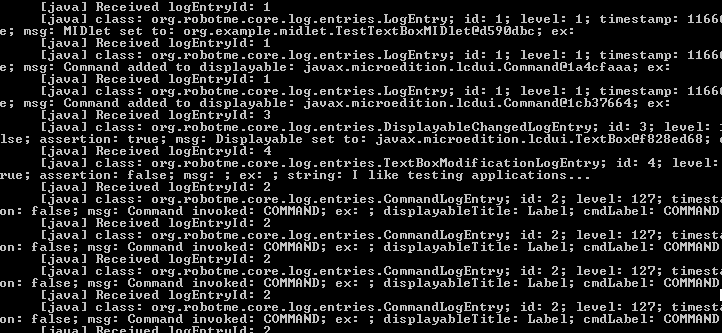
\includegraphics[height=4cm]{figures/2}}\fbox{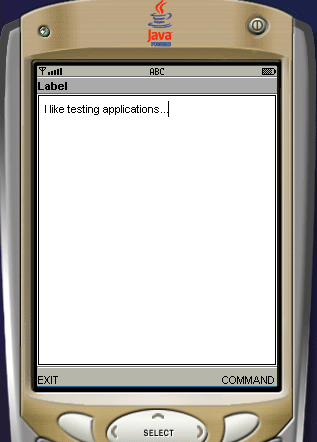
\includegraphics[height=4cm]{figures/1}}
\end{center}
\caption{Screenshots from test recording session. Server console (left) and emulator window (right).}%
\label{fig:session}
\end{figure}

% }}}

\subsection{Replay Phase} % {{{

In the replay phase our `robot' class wraps the original midlet and manages its entire lifecycle. 
The robot continuously reads the binary test script stimulating corresponding events or checking 
for assertion violations. 

There are two types of assertions: strong and weak ones. A failure report is made when any type
of assertion fails, but with strong assertions the simulation is terminated and with
weak ones the program is continued and the robot tries to execute the remaining part of the test script. 
By default all assertions are weak, the test designer may alter their type manually.

Hardware events recorded in the script are generated by the robot back to the tested application in different ways,
depending on their original injection point.

\internalsection{MIDlet Lifecycle.} Midlet lifecycle events are handled much like during recording. The
only difference is that the injected code is instructed to stimulate events (call corresponding
application methods) rather then capture them. One important method is the midlet's startup call (constructor).
The testing framework is interested in intercepting this special call because it is a sign that the replay phase
should begin and the framework should start stimulating events for the application under test.

% We have implemented in our prototype "Intercepting command registration"
% features also in Recording Phase, but I see no advantages of it, it is
% only necessary in Replaying Phase. (further investigation is needed,
% if my assumption is right code needs to be refactored)
\internalsection{Mapping commands to test command identifiers.} During the recording phase every event about a
command the user invoked was recorded. At replay, we simulate the same commands by invoking the
current display listener's \method{commandAction} method. To do so, we must associate previously
recorded commands (or rather their labels) with real objects created during the current test execution
(instances of \texttt{Command} class). We intercept every instance of a command by locating
invocations of the \method{addCommand(Command)} method on subclasses of the \class{Displayable} class. Once
the mapping between the command objects and their labels is known, generation of corresponding test
events only requires the knowledge of a listener where events should be proxied.

\internalsection{Intercepting command listener registration.} Listeners receiving commands from the application
screens register directly with subclasses of the \class{Displayable} class. We intercept these registrations 
by locating all invocations of the \method{set\-Com\-mand\-Listener\-(Command\-Listener)} method. Once we know
which listener registered on the current display, simulation of (previously mapped) command events 
becomes trivial. 

\internalsection{Display changes.} This type of event is tracked during replay (to allow state-change
tracking) in an identical way as in the recording phase. 

\medskip% 
Putting the described code injection procedures together, the testing framework is able to
fully reproduce the original behavior recorded in the test script. The framework performs the
simulation by spawning a background thread that continuously reads events and assertions from the
test script and invokes corresponding event-generation routines, at the same time tracking objects
to which the events should be delegated. While it may seem a bit complex at first glance, the replay
phase is actually quite simple and efficient at runtime.

% }}} // subsection
% }}} // section

\section{Preliminary results} % {{{ 

At the moment of writing, the test framework introduces an overhead of about 30 kilobytes of bytecode
(unobfuscated bytecode). Our estimate is that the overhead will reach about 50 kilobytes
in the final version of the framework. Comparing this figure to storage constraints of present
mobile phones (handling up to a few megabytes) this seems not to be an issue. Runtime memory
consumption increased only about 30 kilobytes (roughly identical to the size of the
code), so it should not be an issue.

The testing framework has different performance overhead depending if it is in the capture or in replay mode. 
In the capture mode the overhead is mostly bound to network traffic (sending events over the wire),
which can be easily neglected by using some engineering tricks (asynchronous queue of events waiting to
be sent). In the replay mode the overhead is connected to the background thread reading and
stimulating events. We found this overhead negligible as well.

The framework has been put to use at NaviExpert (\url{www.naviexpert.pl}), a Polish company offering 
complex navigation software for mobile phones, written entirely in Java. The initial feedback was 
very positive and we plan to collect some usage statistics to determine the value gained
from using regression tests in production use.

We should emphasize that this paper reports on preliminary results from an initial implementation
of the presented concepts. The prototype is fully functional with respect to a large slice of the \jme{}
specification, but does not cover all the possibilities (for example, \class{Canvas} class events
are a matter of future work).

% }}}

\section{Summary and Future Directions} % {{{

We have presented a proof of concept demonstrating that fully-fledged capture-replay testing framework
is feasible in Java 2 Micro Edition environment. The prototype implementation has been well received and
deployed in a commercial software house.

Our biggest challenge at the moment is to provide some objective means to assess the value gained from
using the framework. What common sense states as obvious is quite difficult to express
with hard numbers. We considered a controlled user experiment where participants would be
given the same application and a set of tasks to implement (refactorings and new features). Half of the group would have
access to the results of integration tests, the other half would just work with the code. We hoped this
could demonstrate certain gains (number of early detected bugs, for example) that eventually translate
into economic value for a company. Unfortunately, this kind of experiment is quite difficult to perform
and its results are always disputable (i.e., due to ranging skills between programmers), so we
decided to temporarily postpone it. Other possible research and technical directions are:
%
\begin{itemize}
    \item Design a flexible architecture adding support for events that are outside the scope
    of the \jme{} specification, but are commonly used in mobile development. These events include,
    for example, vendor-specific \acro{api}s such as vibration or backlight by Nokia.

	\item Implement alternative event serialization channels -- through serial cables or Bluetooth 
    connections.

    \item Consider evaluation schemes for the presented solution. A real feedback from
    developers translates into a proof of utilitarian value of the concept -- does the testing 
    framework help? How much time/ work does it save? What is the
    ratio of time spent on recording/ correcting test scripts compared to running them manually? We
    should emphasize that these questions are just as important as they are difficult to answer in a
    real production environment.

	\item Integrate the framework with popular integrated development environments. This
    goal is very important because developers must be comfortable with the tool to use it
    and must feel the benefits it provides. Instant hands-on testing toolkit would certainly assimilate
    faster in the community than an obscure tool (such as Sony's). 

	\item We also think about extending the concepts presented in this paper to other Java-based platforms 
    for building mobile applications, such as NTT DoCoMo Java, BlackBerry RIM API or Qualcomm Brew.
	 They may not be as popular as \jme{}, but the concepts we have presented should be applicable in
	 their case as well.
\end{itemize}

% }}}

\bigskip\noindent\small\textbf{Acknowledgement.}
This work has been partially sponsored by an internal grant  from Poznan University of Technology.

\normalsize\raggedright
\bibliography{references}
\bibliographystyle{splncs}

\section*{Projects surveyed}%
\small
\begin{enumerate}[A.]
    \item \label{j2meunit}%
          J2MEUnit, \url{http://j2meunit.sourceforge.net}.
	\item \label{mobilejunit}%
          Mobile JUnit, Sony Ericsson, \url{http://developer.sonyericsson.com/getDocument.do?docId=87520}.
	\item \label{rational}%
		  TestRT (Rational Test RealTime), IBM, \url{http://www.ibm.com/software/awdtools/test/realtime/}.
	\item \label{bbfledge}%
          Fledge (Java Development Environment and Fledge simulator), Research in Motion,
		  \url{http://na.blackberry.com/eng/developers/downloads/jde.jsp}.
	\item \label{gatling}%
		  Gatling, Motorola, \url{https://opensource.motorola.com/sf/sfmain/do/viewProject/projects.gatling}.
	\item \label{cldcunit}%
		  CLDCUnit, Pyx4me, \url{http://pyx4me.com/snapshot/pyx4me/pyx4me-cldcunit/}.
\end{enumerate}



\end{document}

